\documentclass[12pt,reqno]{amsart}
\usepackage{amsthm,amsmath,amssymb}
\usepackage{mathtools}
\usepackage{proof}
\usepackage{centernot}
\usepackage{xcolor}
\usepackage{graphicx}
\usepackage[T1]{fontenc}
\usepackage{courier}
\usepackage{enumitem}
\usepackage{hyperref}
\hypersetup{
    hidelinks=true
}
\usepackage{array}
\usepackage{multirow}
\usepackage{listings}
\lstset{basicstyle=\ttfamily, columns=fullflexible, language=sql}
\definecolor{mySucces}{RGB}{40, 167, 69}
\definecolor{myFail}{RGB}{220, 53, 69}

\newcommand{\code}[1]{\texttt{#1}}
\newcommand{\st}[0]{\text{ s.t. }}
\newcommand{\where}[0]{\text{ where }}
\newcommand{\mand}[0]{\text{ and }}
\newcommand{\msgspc}[0]{\mathcal{M}}
\newcommand{\cphspc}[0]{\mathcal{C}}
\newcommand{\keyspc}[0]{\mathcal{K}}
\newcommand{\advrs}[0]{\mathcal{A}}
\newcommand{\oracle}[0]{\mathcal{O}}
\newcommand{\correctans}[0]{\colorbox{mySucces}{CORRECT}}
\newcommand{\falseans}[0]{\colorbox{myFail}{FALSE}}
\newcommand\MyBox[2]{
  \fbox{\lower0.75cm
    \vbox to 1.7cm{\vfil
      \hbox to 1.7cm{\hfil\parbox{1.4cm}{#1\\#2}\hfil}
      \vfil}%
  }%
}
\graphicspath{ {./} }
\newtheorem{theorem}{Theorem}[section]
\newtheorem{axiom}[theorem]{Axiom}
\newtheorem{case}[theorem]{Case}
\newtheorem{claim}[theorem]{Claim}
\newtheorem{conclusion}[theorem]{Conclusion}
\newtheorem{condition}[theorem]{Condition}
\newtheorem{conjecture}[theorem]{Conjecture}
\newtheorem{corollary}[theorem]{Corollary}
\newtheorem{criterion}[theorem]{Criterion}
\newtheorem{definition}[theorem]{Definition}
\newtheorem{example}[theorem]{Example}
\newtheorem{exercise}[theorem]{Exercise}
\newtheorem{lemma}[theorem]{Lemma}
\newtheorem{notation}[theorem]{Notation}
\newtheorem{problem}[theorem]{Problem}
\newtheorem{proposition}[theorem]{Proposition}
\newtheorem{remark}[theorem]{Remark}
\newtheorem{solution}[theorem]{Solution}
\newtheorem{summary}[theorem]{Summary}    
\begin{document}

\begin{center}
\large\textbf{Homework 1 \\ COMP530 Fall 2020 - Data Privacy and Security \\}
\normalsize\textbf{ Erhan Tezcan 0070881 \\ 10.11.2020} \\
\end{center}

\begin{center}
\line(1,0){250}
\end{center}

%
%\begin{enumerate}[label=\alph*]
% \item Explain input, output, and the purpose of each algorithm (Key Generation, Encryption, Decryption). 
% \item What are the key space, the message space, and the ciphertext space?
% \item Formally define the   correctness   requirement of an encryption scheme.
% \end{enumerate}
%

\section{Answers}
\textbf{Answer 1:} Note that our data consists of \textit{hospital visits, health records, test results, prescribed medicine etc.} for each \textit{patient}. These are stored and accessed digitally, both by the hospital intranet (doctors, nurses etc.) and the patients themselves. 
\begin{enumerate}
	\item \textbf{Proactive, not reactive; preventive, not remedial.} We should keep in mind problems and attacks that might happen, before they happen! An example would be: instead of saying ``let's keep hospital visit dates public, and if there is a complaint we will make them private'' you should just keep it private in the first place.
	\item \textbf{Privacy as the default setting.} The patient shouldn't make an explicit decision to keep their data private, instead, it should be set to be private from the start. This is rather related to the principle before. We should always ask the consent of patients if we ever have some sort of need to publicize their data.
	\item \textbf{Privacy should be embedded in the system.} This principle states that the privacy settings should be available from the initial design, and not be added afterwards. In our case, the first production version of our online system should have the privacy functionality in it already. This is also related to the prior principles, as if you have thought of privacy in the first place and added it in your system by default, you have met the requirements of assuring this principle.
	\item \textbf{Full Functionality (win-win).} Keeping the data private should be a benefit for both the hospital and the patient. Indeed, there is no reasonable way to argue that keeping these private would be of any harm to anyone!
	\item \textbf{End-to-end Security; Full life-cycle Protection.} Privacy should be enforced from the birth of the data to death. In our case, the patient data is persistent, and should not be erased at all. The moment of creation is when the patient is first adapted to the hospital.
	\item \textbf{Visibility \& Transparency.} Interested parties should have some access to this data. An example of this would be that if a patient is transferred to another hospital with perhaps better equipment or better doctors, then that hospital should have access to the patient's data that which we stored in our hospital. 
	\item \textbf{Keep it user-centric, respect the user.} Our methods should always be in compliance with user's demands and desires. We should always have their consent!
\end{enumerate}
All together, a system where all patient records are stored privately (by default) with respect to the patient-doctor-nurse tuples, where the access is given with respect to the need of this tuple, would be covering all 7 principles. The tuple is important because every treatment or diagnosis requires some sort of prior knowledge (allergy to drugs, past operations etc.). One issue regarding this domain is that, to ask for patient's consent is rather easier on lightweight treatments, because most people would just want to be done with it and get treated. This does assure the last principle, however does the patient fully understand the power of this consent, which they just signed during that treatment?

\vspace{20px}

\textbf{Answer 2:} 
\begin{itemize}
	\item \textbf{Honest-but-curious Doctor}: Indeed, the patients history is stored entirely in the system, however a patient can see more than one doctor in the hospital overall, for example say a patient sees both a Neurolog for some psychological problems and a cardiolog for routine heart checkups. An honest cardiolog doctor might wonder what these psychological problems are, and try to query them from the system. However, this could be prevented by adding additional authorization levels that are with finer granularities: instead of patient-nurse-doctor tuples we could look at patient-nurse-doctor-doctorDomain-patientIllnessDomain etc. to avoid other doctors to peek into our unrelated illnesses.
	\item \textbf{Malicious Nurse}: A nurse can give the patient some drug but record in the system another! Or, they could record the treatment as something else, I actually have a real life example for this which ended up in a fight at the reception, speaking from third person: A patient could go to see the doctor for consult, for example where to go what to do regarding back pain, but no treatment or check-up would made during that meeting. However, the nurse who records the meeting notes it as a ``full-body checkup'' and asks the full price from the patient. This shouldn't be a problem because user will oblige and we should follow their obligation as per last principle, however in practice, who would the hospital trust: one that makes them money or one that does not?
	\item \textbf{Honest-but-curious Mother}: A patient's mother could ask for patient's private hospital records, though in our designed system this shouldn't cause any issues. Since we assume the mother is honest, we assure that they wouldn't lie or something to obtain patient's data, however even if they did, nothing would (or should) be leaked without patient's consent.
	\item \textbf{Man-in-the-Middle}: Though every system is automated to some extent, there is always the need for manual input. This elicits the need of a ``reception desk'' which we are all accustomed to, as per our many hospital visits. You will almost always go to the desk, notify about your arrival, your treatment, or an appointment. Since we want the system to store such things, we would need them to be input to the system, however we should not expect all patients to use a computer and know how to use the system, so this job is done by someone else. In short, the creation of the data includes a third party, in addition to doctor and the patient, and this third party, once creating the data, should not be able to view these data whenever they want. A MITM attack vector is this particular third party, where if they are malicious during the creation of data, the patient wouldn't know about it!
\end{itemize}

\vspace{20px}

\textbf{Answer 3:} 
\begin{enumerate}[label=\alph*.]
	\item This dataset has 11 attributes: \textit{age, workclass, education, marital-status, occupation, relationship, race, gender, hours-per-weel, native-country,} and \textit{income}. 
 	\item The initial dataset has the shape (48842, 11), and after cleaning up it has (45222, 11). This means that 3620 rows were dropped.
 	\item The histgoram is given in figure 1.
 	\begin{figure}
 	\label{fig:hist}
 	\caption{Number of people with income $>$ 50K with respect to their education level.}
 	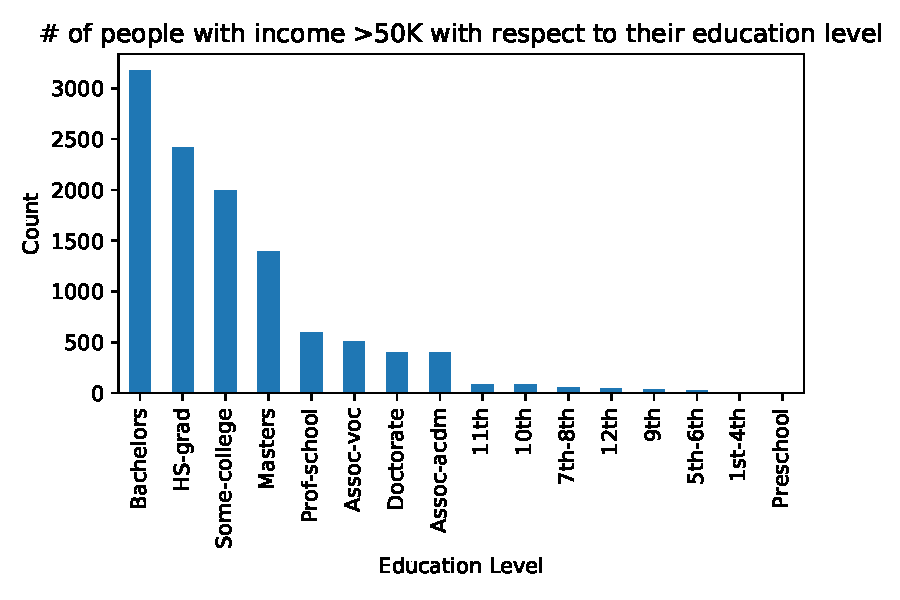
\includegraphics[width=\linewidth]{img/histogram.pdf}
	 \end{figure}
	 	 	
 	\item For this question I will give my answers verbally:
 	\begin{itemize}
 		\item $\text{Pr}[\text{income}>50\text{K }|\text{ race }=\text{ White}]$ is given by \textit{\# of White people with $>$50K income over \# of White people}.
 		\item $\text{Pr}[\text{income}>50\text{K }|\text{ race }=\text{ Black}]$ is given by \textit{\# of Black people with $>$50K income over \# of Black people}.
 		\item $\text{Pr}[\text{income}>50\text{K }|\text{ race }=\text{ Asian-Pac-Islander}]$ is given by \textit{\# of Asian-Pac-Islander people with $>$50K income over \# of Asian-Pac-Islander people}.
 		\item $\text{Pr}[\text{income}\leq50\text{K }|\text{ race }=\text{ White}]$ is given by \textit{\# of White people with $\leq$50K income over \# of White people}.
 		\item $\text{Pr}[\text{income}\leq50\text{K }|\text{ race }=\text{ Black}]$ is given by \textit{\# of Black people with $\leq$50K income over \# of Black people}.
 		\item $\text{Pr}[\text{income}\leq50\text{K }|\text{ race }=\text{ Asian-Pac-Islander}]$ is given by \textit{\# of Asian-Pac-Islander people with $\leq$50K income over \# of Asian-Pac-Islander people}.
 	\end{itemize}
	Note that the last 3 is actually the complement of first three in their respective order, because $Pr[B | A] + Pr[\neg B | A] = 1$, which we will also observe in our results. 
 	
 	\item The results are obtained from my code, which you may find in the submission (\code{q3.py}).
 	\begin{itemize}
 		\item $\text{Pr}[\text{income}>50\text{K }|\text{ race }=\text{ White}] = 0.2623705112716243$
 		\item $\text{Pr}[\text{income}>50\text{K }|\text{ race }=\text{ Black}] = 0.12630085146641437$  
 		\item $\text{Pr}[\text{income}>50\text{K }|\text{ race }=\text{ Asian-Pac-Islander}] = 0.2831926323867997$  
 		\item $\text{Pr}[\text{income}\leq50\text{K }|\text{ race }=\text{ White}] = 0.7376294887283757$ 
 		\item $\text{Pr}[\text{income}\leq50\text{K }|\text{ race }=\text{ Black}] = 0.8736991485335857$  
 		\item $\text{Pr}[\text{income}\leq50\text{K }|\text{ race }=\text{ Asian-Pac-Islander}] = 0.7168073676132003$ 
 	\end{itemize}
 	There are 38903 white people (10207 high income, 28696 low income), 4228 black people (534 high income, 3694 low income) and 1303 asian-pac-islander people (369 high income, 934 low income).
 	
 	\item The question at hand was to see if whether somebody's race is related to their income. Indeed we see that black people seem to be less probable to have high income compared to the other two races, however, neither this dataset alone could indicate it nor this conditional probably would suffice. Income has many factors, such as education, occupation and country. Also, asian-pac-islander people seem to have higher probability of having income compared to white people, but notice that we are calculating this over 38K white people versus just 1.3K asian-pac-islander people. 
\end{enumerate}

\vspace{20px}

\textbf{Answer 4:} Ali has 1000 login attempts, of which 865 are positive. However, he claims he only made 900 attempts, and he was able to login 850 times. In the table 1 we see the situation:
\begin{table}[]
\begin{tabular}{|l|l|l|l|}
\hline
\multicolumn{1}{|c|}{} &
  \multicolumn{1}{c|}{\begin{tabular}[c]{@{}c@{}}Ali\\ attempts\end{tabular}} &
  \multicolumn{1}{c|}{\begin{tabular}[c]{@{}c@{}}Someone else\\ attempts\end{tabular}} &
  $\Sigma$ \\ \hline
Login  & 850 & 15  & 865  \\ \hline
Reject & 50  & 85  & 135  \\ \hline
$\Sigma$   & 900 & 100 & 1000 \\ \hline
\end{tabular}
\caption{Biometric authentications of Ali's retina scanner.}
\label{tab:aliattempts}
\end{table}
We have: $TP=850$, $FP=15$, $FN=50$, $TN=85$. The formulas below are taken from wiki.\footnote{https://en.wikipedia.org/wiki/Sensitivity\_and\_specificity}
\begin{itemize}
	\item Sensitivity, recall, hit rate or true positive rate (TPR):
	$$
	\frac{TP}{TP+FN}=\frac{850}{850+50}=0.9444
	$$
	\item Specificity, selectivity or true negative rate (TNR):
	$$
	\frac{TN}{TN+FP}=\frac{85}{85+15}=0.85
	$$
	\item Precision or positive predictive value (PPV):
	$$
	\frac{TP}{TP+FP}=\frac{850}{850+15}=0.9823
	$$
	\item Accuracy:
	$$
	\frac{TP+TN}{TP+TN+FP+FN}=\frac{850+85}{850+85+15+50}=0.9350
	$$
	\item F1 Score:
	$$
	\frac{2TP}{2TP+FP+FN}=\frac{2\times850}{2\times850+15+50}=0.9632
	$$
\end{itemize}
\vspace{20px}

\textbf{Answer 5:}
\begin{enumerate}[label=\alph*.]
	\item The CSV file \code{rockyouDictionary.csv} and the source code \code{q5.py} are attached in the submission.
	\item Alice's password is \code{iloveyou2}, Bob's password is \code{gangsta}, and Charlie's password is \code{beautiful}.
	\item The attack from parts (a) and (b) work. What we are doing is also known as a preimage attack, where given a hash function $H : X \xrightarrow{} Y$ (\code{sha512}) and $y \in Y$ (user's password hash), we are trying to find an $x \in X$ (user's actual password) such that $H(x)=y$. The thing is, what normally would be the entire domain $X$ of this function, is narrowed down to a bare few hundred elements in \code{rockyou.txt}, which enables us to try all of these and see if we can succeed in our preimage attack. Indeed, we were able to find the passwords, which is due to the fact that Alice, Bob and Charlie used popular passwords, which we had in our dictionary!
	\item Our attack will be similar to the one we did above, however it will have a twist. Let $P$ be the set of passwords we will have in our dictionary (as obtained from \code{rockyou.txt}). Let $H$ be the hash function. Our dictionary included the result of these hash functions, as $P \implies H(P)$. Now, we will have to consider the salt. We know that the trick is to do \code{password || salt} and take the hash of this. Let $S$ be the set of salts to consider (as obtained from \code{salty-rockyou.txt}), now we will calculate the dictionary as $P \times S \implies H(P \times S)$, where for $p \in P$ and $s \in S$, $p \times s = p || s$. Our dictionary was normally of size $|P|$, but now it will be $|P|\times|S|$. This requires $|S|$ times more computation than the previous attack.
	\item Dave's password is \code{manutd}, Elaine's password is \code{hello}, and Faith's password is \code{0123456789}. The source code \code{q5.py} is attached in submission.
\end{enumerate}


\vspace{20px}

\textbf{Answer 6:}
\begin{enumerate}[label=\alph*.]
	\item Note that here we could have a group called \code{NEW\_EMPLOYEE} with such privileges and add Frank to this group.
	\begin{lstlisting}[language=sql]
GRANT INSERT INTO
ON STUDENTS
TO Frank
	\end{lstlisting}
	\item 
	\begin{lstlisting}[language=sql]
GRANT ALL
ON COURSES
TO Jill
	\end{lstlisting}
	\item
	\begin{lstlisting}[language=sql]
REVOKE ALL
ON *
FROM Frank
	\end{lstlisting}
	\item
	\begin{lstlisting}[language=sql]
GRANT UPDATE (capacity)
ON COURSES
TO Matthew
	\end{lstlisting}
\end{enumerate}



\end{document}